\documentclass[a4paper]{article}

\usepackage[english]{babel}
\usepackage[utf8]{inputenc}
\usepackage{amsmath}
\usepackage{graphicx}
\usepackage[colorinlistoftodos]{todonotes}

\title{TTM4100 \\ Prosjektøving 1}

\author{Gruppe 31 \\\\ Bård Schjander Flugon \\ Neshat Naderi \\ Kristian Fladstad Normann \\ Stian Hegerland Hagen \\ Markus Lund \\ Kristian Bjørn Thoresen}

\date{\today}


\begin{document}
\maketitle
\clearpage

\section*{Klassediagram}
\label {sec:class}

\begin{figure}[ht]
\centering
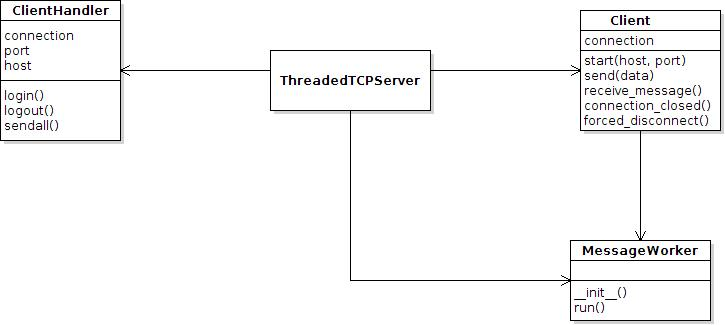
\includegraphics[width=1\textwidth]{classDiag.jpg}
\caption{\label{fig:classDiag}Klassediagram}
\end{figure}



\section*{Sekvensdiagram}
\label{sec:sek}

\begin{figure}[ht]
\centering
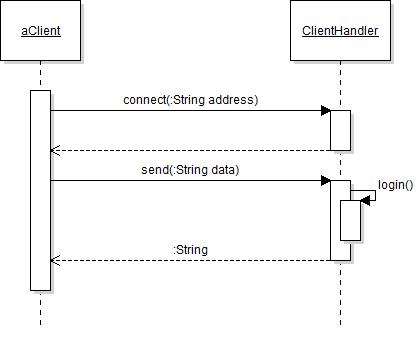
\includegraphics[width=1\textwidth]{loginSeq.jpg}
\caption{\label{fig:loginSeq}Login.}
\end{figure}

\begin{figure}[ht]
\centering
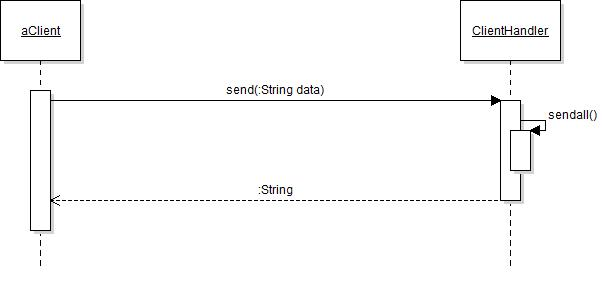
\includegraphics[width=1.3\textwidth]{msgSeq.jpg}
\caption{\label{fig:msgSeq}Sende melding.}
\end{figure}

\begin{figure}[ht]
\centering
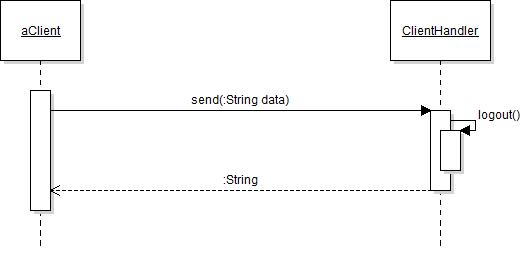
\includegraphics[width=1.2\textwidth]{logoutSeq.jpg}
\caption{\label{fig:logoutSeq}Logout.}
\end{figure}
\clearpage

\section*{}



\end{document}
